% =====================================================================================
% Revision sections answering the review (heterogeneity evidence, baselines, task scope,
% metric choice, what FL contributes). Drop into the Overleaf project:
%   - Sec. 1 replaces the task list / RQs in the Introduction
%   - Sec. 2 is a new paragraph + table for Related Work
%   - Sec. 3 goes after "Datasets and Data Cleaning" (needs fig_heterogeneity.pdf)
%   - Sec. 4 replaces the "Evaluation" paragraph of the Methodology
%   - Sec. 5 is new Results subsections; cells marked \tbd are filled from the revision runs
%     (python run_queue.py --plan revision ...; python scripts/significance.py ...)
% Bib entries: references_additions.bib (new ones at its end).
% Packages: booktabs, graphicx, amsmath, amssymb (\checkmark), xcolor (\textcolor).
% =====================================================================================
\newcommand{\tbd}{\textcolor{gray}{--}}

% -------------------------------------------------------------------------------------
\subsection*{[Intro] Scope: three tasks}
We restrict the study to three tasks that share one input (the judgment text with its operative
ending removed) and one model: \textbf{case duration} (Task~1, regression on $\log(1+\text{days})$),
\textbf{case type} (Task~2, ten families) and \textbf{disposal nature} (Task~3, allowed / dismissed /
disposed of / withdrawn). Constitutional-article prediction and past-case retrieval, listed in the
proposal, are dropped: their labels are sparse in the High Court sample (the Constitution is cited in
3\% of Bombay judgments), retrieval needs a different model and evaluation (Supreme Court corpus, AILA,
IL-PCSR) and would not share the federated encoder, and statute and precedent retrieval on Indian data
is already covered by centralized benchmarks such as IL-TUR~\cite{joshi2024iltur}. The three remaining
tasks form a cascade (case type $\rightarrow$ disposal) and are the ones on which courts differ most,
which is the question federated learning has to answer.

Research questions (revised):
\begin{enumerate}
  \item[RQ1] Are the courts measurably non-IID, and in which of the three tasks?
  \item[RQ2] Does federated training beat what a court can do alone, and how does it compare with
             existing federated algorithms, including those benchmarked in FedLegal~\cite{zhang2023fedlegal}?
  \item[RQ3] What does federation give a court that it cannot get alone: help when its own data are
             scarce, and a usable model for a court that has no labelled data?
\end{enumerate}

% -------------------------------------------------------------------------------------
\subsection*{[Related work] Positioning against FedLegal and IL-TUR}
FedLegal~\cite{zhang2023fedlegal} is the closest work: a federated benchmark for legal NLP on Chinese
court data, where each task is trained with standard FL algorithms and the conclusion is that real
legal non-IID data hurt FL. IL-TUR~\cite{joshi2024iltur} is the standard benchmark for Indian legal
text understanding (named-entity recognition, rhetorical roles, judgment prediction with explanation,
bail prediction, statute identification, prior-case retrieval, summarisation, translation), with
centralized training only. Table~\ref{tab:novelty} lists what each covers. Our study differs in three
ways: (i) it is the first federated study on Indian court data, with the court as the natural client,
(ii) it asks questions neither benchmark has (case duration, a regression task, and case type and
disposal predicted jointly in a multi-task cascade), and (iii) it proposes methods for the multi-task
non-IID setting (TSR and PTM) and compares them with the FedLegal-style algorithm suite inside one
code base, under the same encoder, data and budget.

\begin{table}[h]\centering\small
\begin{tabular}{@{}lccc@{}}\toprule
 & FedLegal & IL-TUR & Ours \\ \midrule
Jurisdiction & China & India (mostly SC) & India, 5 High Courts \\
Federated training & \checkmark & -- & \checkmark \\
Natural clients (courts) & \checkmark & -- & \checkmark \\
Quantified heterogeneity & partly & -- & \checkmark\ (Sec.~\ref{sec:hetero}) \\
Case duration (regression) & -- & -- & \checkmark \\
Case type + disposal, multi-task cascade & -- & -- & \checkmark \\
Judgment / bail prediction & \checkmark & \checkmark & disposal nature \\
Personalised / per-task sharing & -- & -- & \checkmark\ (PTM) \\
Unseen-court evaluation & -- & -- & \checkmark \\ \bottomrule
\end{tabular}
\caption{What each benchmark covers. IL-TUR tasks and our tasks do not overlap, so numbers are not
directly comparable; the comparison with FedLegal is made by running its algorithm suite on our data
(Table~\ref{tab:fedlegal}).}
\label{tab:novelty}
\end{table}
% CHECK before submitting: the exact algorithm list and the non-IID analysis in the FedLegal paper
% (ACL 2023, Sec. 4-5), and the IL-TUR task list (ACL 2024). The cells above follow the papers'
% abstracts; adjust "partly" if FedLegal reports a quantitative non-IID statistic.

% -------------------------------------------------------------------------------------
\section{Evidence that the courts are non-IID}
\label{sec:hetero}
Federated-learning papers distinguish four kinds of client heterogeneity~\cite{kairouz2021advances}:
different amounts of data (quantity skew), different label distributions $P_k(y)$ (label skew),
different inputs $P_k(x)$ (covariate shift) and different input--label relations $P_k(y\mid x)$
(concept shift). We test each on the 12,360 judgments used to train and evaluate the models
(Table~\ref{tab:hetero}, \texttt{scripts/heterogeneity\_stats.py}). The text sample has about 2,500
judgments per court by design, so quantity skew is measured on all 284,405 decisions of 2024 in the
eCourts metadata instead: the largest court there has 7.5 times the cases of the smallest.

\begin{table}[h]\centering\small
\begin{tabular}{@{}llll@{}}\toprule
Kind & Test & Statistic & Effect size \\ \midrule
Label: duration & Kruskal--Wallis on $\log(1+\text{days})$ & $H=555$, $p<10^{-100}$ & $\varepsilon^2=0.045$; mean pairwise KS $D=0.21$ \\
Label: duration class & $\chi^2$ court $\times$ 4 classes & $\chi^2_{12}=743$, $p<10^{-100}$ & Cram\'er's $V=0.14$ \\
Label: case family & $\chi^2$ court $\times$ 10 families & $\chi^2_{36}=4{,}045$, $p<10^{-300}$ & $V=0.29$; mean pairwise JSD $=0.15$ \\
Label: disposal & $\chi^2$ court $\times$ 4 outcomes & $\chi^2_{12}=808$, $p<10^{-100}$ & $V=0.15$; mean pairwise JSD $=0.03$ \\
Concept: duration $\mid$ type & two-way ANOVA, court $\times$ family & $F_{12}=39.4$, $p<10^{-90}$ & $R^2$: $0.028\rightarrow0.127$ with court \\
Concept: disposal $\mid$ type & $\chi^2$ court $\times$ outcome within family & $\chi^2_{69}=1{,}648$, $p<10^{-290}$ & median $V=0.22$ (8 families) \\
Covariate: text & court identification from masked text & 99.97\% vs 20\% chance & binomial $p<10^{-300}$ \\
Transfer & train on court $i$, test on court $j$ & MAE$_{\log}$ $1.32\rightarrow2.01$ & disposal F1 $0.65\rightarrow0.25$ \\ \bottomrule
\end{tabular}
\caption{Heterogeneity tests on the 12,360 judgments used in the experiments. JSD: Jensen--Shannon divergence
(base 2, 0 = identical). Transfer: TF-IDF linear models, own court (diagonal) vs other courts (off-diagonal).}
\label{tab:hetero}
\end{table}

\begin{figure}[h]\centering
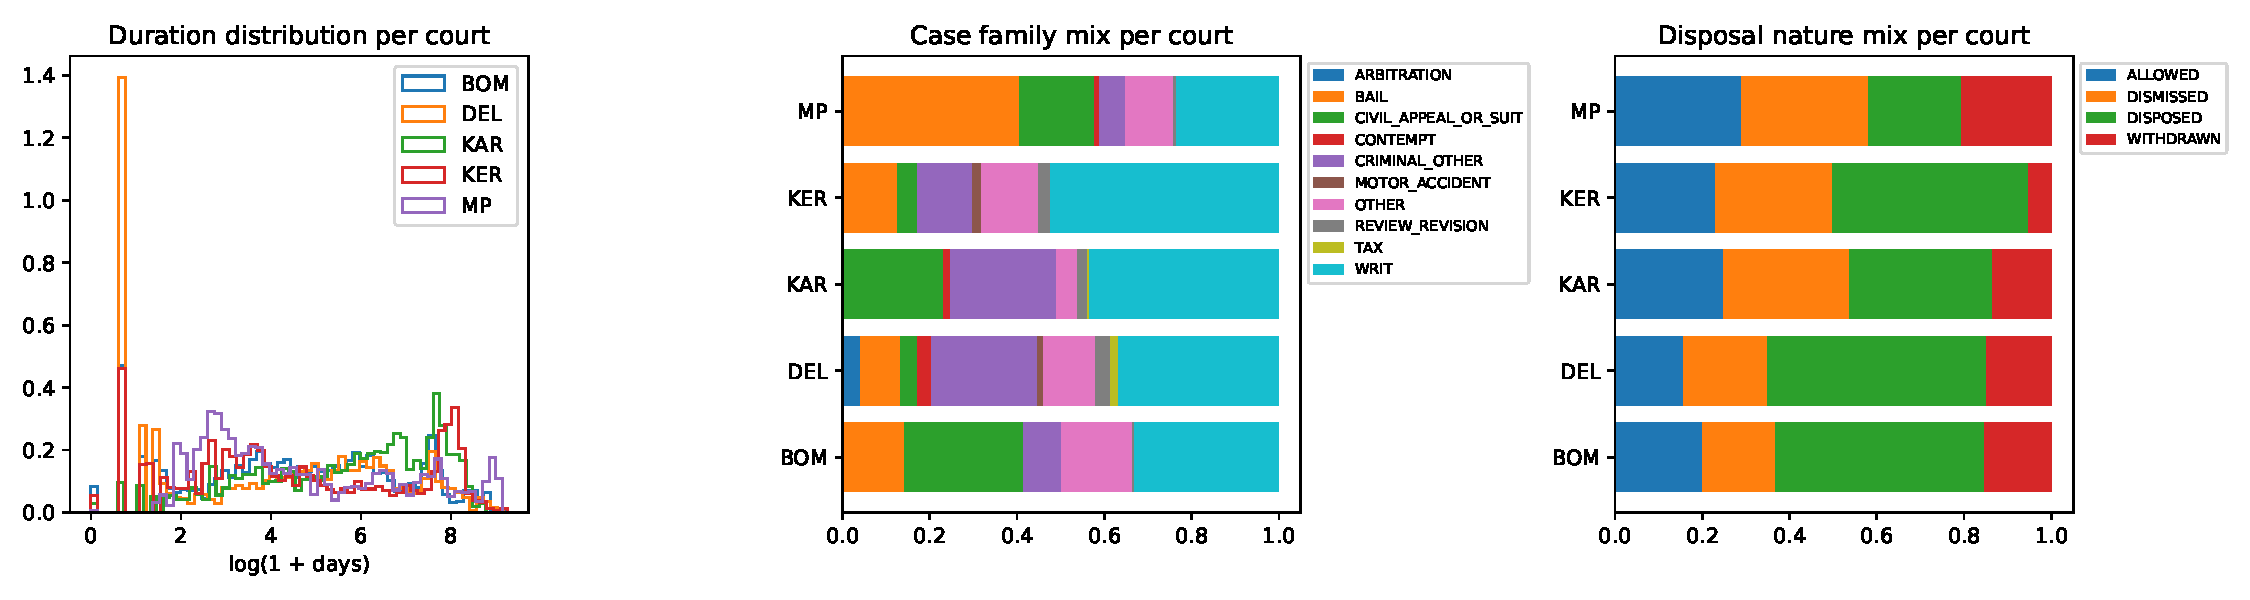
\includegraphics[width=\linewidth]{fig_heterogeneity.pdf}
\caption{Per-court distributions of case duration, case family and disposal nature (text sample).}
\label{fig:hetero}
\end{figure}

\textbf{All kinds of skew are present and statistically significant.} Because $p$-values shrink with
sample size, the effect sizes carry the argument, and they lead to three conclusions.

\emph{(1) The label skew is real but moderate.} Case families differ most between courts (Cram\'er's
$V=0.29$): Madhya Pradesh is dominated by bail matters, Kerala by writs. The outcome mix differs less
($V=0.15$). To compare with the synthetic splits used in FL papers, we found the Dirichlet
concentration whose simulated clients are as far from the pooled label distribution as the real
courts~\cite{hsu2019fedavgm}. Case families match $\mathrm{Dir}(\alpha\approx1.6)$ per class and
disposal $\mathrm{Dir}(\alpha\approx10)$; common FL benchmarks use $\alpha=0.1$--$0.5$. Label skew
alone therefore does not explain why plain FedAvg falls behind local training.

\emph{(2) The concept shift is what hurts a shared model.} The same case family takes a different time
in each court: case family alone explains 2.8\% of the variance in log-duration, and adding the court
and the court$\times$family interaction raises this to 12.7\%. Within a family the outcome mix still
depends on the court (median $V=0.22$; $V=0.35$ for bail). A model trained on one court and applied
to another loses 0.69 MAE$_{\log}$ on duration (a factor $e^{0.69}\approx2$ in days) and
62\% of its disposal F1.

\emph{(3) The inputs differ too.} After masking places, numbers and dates, a linear classifier
identifies the court of a judgment with 99.97\% balanced accuracy. Most of the telling features are
drafting conventions: ``through Mr'' and ``coram'' in Delhi, ``by Sri'' and ``praying'' in Karnataka,
``the honourable'' and ``aged \ldots\ years'' in Kerala, ``by Shri'' in Madhya Pradesh, ``of
judicature at'' in Bombay. A few are residual identifiers (bench abbreviations, PIN codes), so the
figure is an upper bound on the pure style difference.

These results predict which parts of the model should be shared. Case type is recorded and drafted
in a court-specific way, so its head should stay local. Duration depends on the court for the same
case type, so it needs a shared encoder plus a court-aware head. PTM's learned weights recover exactly
this ordering without being told (Section~\ref{sec:ptmw}).

\subsection*{[Methodology] Evaluation: one primary metric per task, one headline number}
We report one primary metric per task:
\begin{itemize}
  \item \textbf{Duration: MAE on $\log(1+\text{days})$.} It is a relative error (an MAE$_{\log}$ of 0.5
        means predictions are off by a factor $e^{0.5}\approx1.65$ in days), so a 30-day bail matter and a
        five-year civil appeal count equally. It is not dominated by the long tail (durations reach
        13,840 days), it matches the training loss, and it is defined per court. Spearman correlation
        only measures ranking, and the four-class F1 depends on arbitrary bucket edges, so both are
        moved to the appendix.
  \item \textbf{Case type and disposal nature: macro-F1.} The classes are imbalanced and their mix
        differs by court (Table~\ref{tab:hetero}), so accuracy would reward predicting each court's
        majority class. Macro-F1 weights every class equally.
\end{itemize}
To rank methods with \emph{one} number we use the standard multi-task measure
$\Delta_{\text{MTL}}$~\cite{maninis2019attentive,vandenhende2021mtl}, the mean relative improvement
over local-only training across the three tasks:
\begin{equation}
\Delta_{\text{MTL}} = \frac{100}{3}\sum_{t=1}^{3} s_t\,\frac{M_t - M_t^{\text{local}}}{M_t^{\text{local}}},\qquad
s_t=-1 \text{ for MAE}_{\log},\; +1 \text{ for F1}.
\end{equation}
The reference is local-only training because it answers the question a court faces: is joining the
federation better than training alone? $\Delta_{\text{MTL}}>0$ means yes, averaged over tasks. We
report it for the mean over courts and for the \textbf{worst court}, because a federation that helps on
average while hurting one member is not acceptable to that member. Significance is tested with paired
Wilcoxon tests over the 15 (court, seed) pairs and with a case-level paired bootstrap within each court
(\texttt{scripts/significance.py}).

% -------------------------------------------------------------------------------------
\section*{[Results] Revised results}
All rows use InLegalBERT with LoRA, the TSR input (first and last 256 tokens), the same rounds and early
stopping, and three seeds unless stated otherwise. $\Delta_{\text{MTL}}$ is relative to local-only
training with the same model; the worst-court column is the lowest per-court $\Delta_{\text{MTL}}$.
Paired tests are Wilcoxon signed-rank tests over the 15 (court, seed) pairs.

\subsection*{Comparison with the FedLegal algorithm suite and with centralized training}
\begin{table}[h]\centering\small
\begin{tabular}{@{}lcccccc@{}}\toprule
Method & MAE$_{\log}\downarrow$ & Type F1$\uparrow$ & Disp. F1$\uparrow$ & $\Delta_{\text{MTL}}$ (\%) & Worst court (\%) & $p$ vs ours \\ \midrule
\multicolumn{7}{@{}l}{\emph{No collaboration}} \\
Local only & 1.371 & 0.873 & 0.533 & 0.00 & 0.00 & 0.015 \\ \midrule
\multicolumn{7}{@{}l}{\emph{Federated, one shared model (FedLegal-style)}} \\
FedAvg~\cite{mcmahan2017communication}$^\dagger$ & 1.347 & 0.844 & 0.539 & $-0.15$ & -- & -- \\
FedProx~\cite{li2020federated} & 1.383 & 0.775 & 0.532 & $-4.05$ & $-9.26$ & $<0.001$ \\
FedAdam~\cite{reddi2021adaptive} & 1.369 & 0.792 & 0.526 & $-3.44$ & $-6.94$ & $<0.001$ \\ \midrule
\multicolumn{7}{@{}l}{\emph{Federated, personalised}} \\
FedPer (all heads local)~\cite{arivazhagan2019fedper} & 1.375 & 0.913 & 0.556 & $+2.86$ & $-1.99$ & 0.17 \\
Ditto ($\lambda=1$, chosen on val.)~\cite{li2021ditto} & \textbf{1.329} & 0.872 & 0.555 & $+2.40$ & $-0.29$ & 0.15 \\
TSR + PTM, before fine-tuning & 1.376 & 0.914 & 0.556 & $+2.93$ & $-0.93$ & 0.21 \\
\textbf{TSR + PTM + ft (ours)} & 1.359 & \textbf{0.917} & 0.559 & $+3.60$ & $+0.62$ & -- \\ \midrule
\multicolumn{7}{@{}l}{\emph{Centralized (pooled data, IL-TUR-style; not private)}} \\
Centralized & 1.358 & 0.860 & 0.559 & $+1.48$ & $-3.92$ & -- \\
Centralized + per-court ft & 1.333 & 0.906 & \textbf{0.568} & $\mathbf{+4.42}$ & $\mathbf{+1.31}$ & 0.30 \\ \bottomrule
\end{tabular}
\caption{Main comparison (TSR model, 3 seeds, test set, mean over courts). $^\dagger$From the earlier runs (3 seeds,
Table~7 of the first version), not re-run; $\Delta_{\text{MTL}}$ computed against the local reference above. SCAFFOLD~\cite{karimireddy2020scaffold} diverged
($\Delta_{\text{MTL}}=-37\%$) with our AdamW local optimizer, whose adaptive steps break SCAFFOLD's
SGD-based drift correction; it is not reported further.}
\label{tab:main}
\end{table}

Table~\ref{tab:main} gives four findings.
\begin{enumerate}
  \item \textbf{Generic federated algorithms do not help on these courts.} FedProx and FedAdam end
        3--4\% \emph{below} local training, and their worst court loses 7--9\%. Almost all of the loss is
        in case type (F1 0.77--0.79 against 0.87 locally), which every court records in its own way
        (Section~\ref{sec:hetero}). This reproduces FedLegal's observation that real legal non-IID data
        hurt standard FL, now on Indian courts and with the cause identified.
  \item \textbf{Personalised federation beats training alone.} Our method improves on local training by
        $\Delta_{\text{MTL}}=+3.6\%$ (Wilcoxon $p=0.015$), significantly in case type ($p=0.012$, better
        in all five courts) with a smaller gain in disposal ($p=0.08$). It is the only federated method
        whose worst court also improves ($+0.6\%$). It beats FedProx and FedAdam by 9--10\% ($p<0.001$).
  \item \textbf{Our method ties the other personalised methods.} The differences from FedPer
        ($p=0.17$) and Ditto ($p=0.15$) are not significant. Ditto has the lowest duration error,
        ours the best case type. What PTM adds is not accuracy but interpretable, per-court and
        per-task sharing weights (below), learned in one training stage.
  \item \textbf{Federation matches centralized training without pooling the data.} Centralized
        training with the same per-court fine-tuning is $0.6\%$ ahead, which is not significant
        (Wilcoxon $p=0.30$; the case-level bootstrap 95\% intervals of the difference include zero for
        every metric in each of the three seeds).
        Plain centralized training without fine-tuning is $2.1\%$ \emph{behind} ours. Pooling the
        five courts' judgments therefore buys little accuracy over keeping them in place.
\end{enumerate}

\subsection*{Is TSR more than extra context?}
A single-view model reading the first and last 256 tokens (512 in total) does as well as TSR:
local training reaches MAE$_{\log}$ 1.347 and $\Delta_{\text{MTL}}=+3.7\%$, statistically tied with
ours ($p=0.98$), and FedAvg + ft at 512 tokens gives $+3.2\%$ ($p=0.33$ vs ours). The duration gain
reported for TSR in the earlier version therefore comes mostly from reading more of the judgment,
not from the task-specific weighting. TSR remains useful for interpretation: it shows that case type
is read from the start of a judgment, disposal from the end, and duration from both
(Figure~\ref{fig:segw}).

\subsection*{What the learned sharing weights show}
\label{sec:ptmw}
The PTM weight on the shared head is stable across seeds and orders the tasks the same way in every
court: duration 0.34--0.44, disposal 0.15--0.20, case type 0.04--0.08 (std over seeds $\le0.10$).
Courts rely on collaboration most for duration and hardly at all for case type, which is the ordering
predicted by the heterogeneity tests.

\subsection*{What federation gives a court}
\textbf{Low-resource courts.} Each court keeps only 10\%, 25\% or 50\% of its training judgments
(about 175, 440 and 875 cases; one seed).

\begin{table}[h]\centering\small
\begin{tabular}{@{}lccccc@{}}\toprule
Data per court & Local MAE$_{\log}$ / type F1 & Federated MAE$_{\log}$ / type F1 & Fed. $\Delta_{\text{MTL}}$ (\%) & Centralized $\Delta_{\text{MTL}}$ (\%) \\ \midrule
10\% & 1.599 / 0.523 & 1.704 / 0.598 & $+2.3$ & $+12.2$ \\
25\% & 1.487 / 0.626 & 1.555 / 0.812 & $+7.3$ & $+10.7$ \\
50\% & 1.403 / 0.808 & 1.439 / 0.881 & $+1.4$ & $-0.8$ \\
100\% (3 seeds) & 1.371 / 0.873 & 1.359 / 0.917 & $+3.6$ & $+1.5$ \\ \bottomrule
\end{tabular}
\caption{Federated (TSR + PTM + ft) and centralized vs local training as each court's data shrink.
$\Delta_{\text{MTL}}$ relative to local training at the same data size. One seed except the last row.}
\label{tab:lowres}
\end{table}

Federation helps most when a court has a few hundred cases: at 25\% it raises case-type F1 from 0.63 to
0.81 and $\Delta_{\text{MTL}}$ by 7.3\%, recovering about two thirds of what pooling the raw data would give.
With very little data (10\%) the gain is mostly case type, while duration becomes worse than local
training (1.70 against 1.60), and pooled training is far ahead ($+12\%$). With half the data the gain
falls to $+1.4\%$. These are single-seed results and should be read as a trend.

\textbf{A court with no labelled data.} Each court in turn is left out of training and only evaluated.
Without federation, it could only borrow another court's local model.

\begin{table}[h]\centering\small
\begin{tabular}{@{}lcccc@{}}\toprule
Held-out court & Mean other court & Best other court & FedAvg, 4 courts & Centralized, 4 courts \\ \midrule
Bombay & $-36.0$ & $-31.3$ & $\mathbf{-25.9}$ & $-28.9$ \\
Delhi & $-49.2$ & $-42.5$ & $\mathbf{-37.7}$ & $-39.0$ \\
Karnataka & $-35.1$ & $-17.3$ & $\mathbf{-15.6}$ & $-30.4$ \\
Kerala & $-52.9$ & $-42.4$ & $\mathbf{-32.8}$ & $-40.8$ \\
Madhya Pradesh & $-51.0$ & $\mathbf{-41.3}$ & $-43.6$ & $-46.0$ \\ \bottomrule
\end{tabular}
\caption{Unseen-court generalisation: $\Delta_{\text{MTL}}$ (\%) relative to the court's own local model
(one seed). ``Best other court'' is chosen with hindsight on the test set.}
\label{tab:unseen}
\end{table}

For four of the five courts, the federated model trained on the other four is the best model a new
court can get, better than the best single other court (chosen with hindsight) and better than
centralized training on the same four courts. The exception is Madhya Pradesh, whose caseload (mostly
bail) is the most unusual. Every option is still 16--44\% worse than the court's own local model, so a
new court should join the federation and fine-tune rather than use the shared model as is.

\subsection*{Revised claims}
\begin{itemize}
  \item The five High Courts are measurably non-IID, mainly through court-specific durations for the
        same case type and court-specific drafting, not through label imbalance alone.
  \item Standard federated algorithms of the kind benchmarked in FedLegal lose to local training on
        these courts. Per-task personalisation is required, and with it federation beats local training
        ($p=0.015$) and is statistically tied with centralized training, without moving any judgment.
  \item Federation helps most for courts with a few hundred labelled cases, and gives a court with
        no labels a better starting model than any single other court in four of five cases.
  \item The proposed PTM is on par with Ditto and FedPer in accuracy and adds interpretable sharing
        weights. The duration gain of TSR comes mostly from reading 512 tokens.
\end{itemize}
